%%%%%%%%%%%%%%%%%%%%%%%%%%%%%%%%%%%%%%%%%%%%%%%%%%%%%%%%%%%%%%%%%%%%%%%%%%%%%%%%
%% MASTER'S THESIS                                                            %%
%%                                                                            %% 
%% Title (en): Multi-Agent Systems and Organizations                          %%
%% Title (cs): Multiagentní systémy a organizace                              %%
%%                                                                            %%
%% Author: Bc. Lukáš Kúdela                                                   %%
%% Supervisor: Prof. RNDr. Petr Štěpánek, DrSc.                               %%
%%                                                                            %%
%% Academic year: 2011/2012                                                   %%
%%%%%%%%%%%%%%%%%%%%%%%%%%%%%%%%%%%%%%%%%%%%%%%%%%%%%%%%%%%%%%%%%%%%%%%%%%%%%%%%

\section{Static Model}

The \textit{static model} is used to model static (structural) aspects of organizations: such as:
\begin{itemize}
	\item an organization's role structure and protocols,
	\item a role's competences and responsibilities, or
	\item a player's capabilities.
\end{itemize}

% Two partitions: functional & technical
The metamodel model can be partitioned in two orthogonal ways: \textit{functional}\comments{FO} and \textit{technical}\comments{FO}.
First, both partitions will be described, and then the integrated static model will be presented.

% Functional partition
The \textit{functional partition} divides the concepts according to the area they represent: organization, player or protocol.
This is a more natural partition of the two, since fewer dependencies among concepts from different parts exists than in the other partition.
The organization/protocol part of the MAS can be designed (and implemented) independently of the player part; indeed agent developed by one team can play roles in organizations developed by another team.

% Technical partition
The \textit{technical partition} separates the concepts based on whether they represent design-time or run-time entities.
The design-time entities are created already at design-time and are usually implemented as \textit{agent classes} in the target agent platform; they are analogous to object classes in OOP.
The run-time entities are created only at run-time and are usually implemented as \textit{agent instances} in the target agent platform; they are analogous to object instances in OOP.

% Type-token distinction - definition
Before continuing with the presentation of \textit{Thespian}, it is important to explain the \textit{type-token distinction}.
In disciplines such as philosophy and knowledge representation, the type-token distinction is a distinction that separates a \textit{concept} from objects that are particular \textit{instances} of that concept \cite{Wikipedia-TTD}.
\textit{Thespian} has been designed to support the type-token distinction and the correct differentiation between types and their tokens is a recurring theme in this chapter.

% Type-token distinction - MAS
As an example of the type-token distinction, consider a MAS.
The \textit{specification} of the MAS (its source code) is a \textit{MAS type} and its \textit{manifestation} (a running MAS) is a \textit{MAS token}.
Just like a type can (and usually does) have many tokens, a MAS specification can have multiple manifestations---the same source code can be run many times, each time yielding a different run.

%%%%%%%%%%%%%%%%%%%%%%%%%%%%%%%%%%%%%%%%%%%%%%%%%%%%%%%%%%%%%%%%%%%%%%%%%%%%%%%%
\subsection{Organization Model}

% Organization model - usage
The \textit{Organization model} (figure~\ref{figure:thespian-organization-model}) contains concepts whose instances model organizations and roles with their competences and responsibilities.

% Figure: Thespian - Organization model
\begin{figure}[ht]
	\centering
	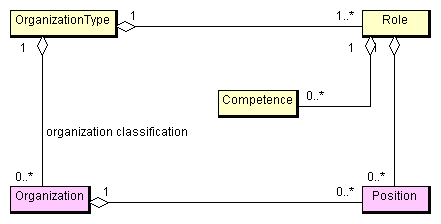
\includegraphics[width=0.6\textwidth]{images/thespian/organization-model}
	\caption{The Organization model}
	\label{figure:thespian-organization-model}
\end{figure}

\subsubsection*{Organization and Organization Type}

% Type-token distinction - organization
To enable the type-token distinction for organizations, \textit{Thespian} contains concepts for modelling both an \textit{organization type} and an \textit{organization token}: \textit{Organization type} and \textit{Organization}.

% Organization type
\textit{Organization type} (also called \textit{Organization class}) is a class of organizations sharing the same role structure; it is a design-time entity.
% Organization type - state
It contains a set of \textit{roles}\comments{FO} defining its role structure.
% Organization type - behaviour
It can be instantiated to yield an \textit{organization}\comments{FO}.

% Organization
\textit{Organization} (also called \textit{Organization instance}) is an actual organization in a running MAS; it is a run-time entity.
% Organization - state
It is classified by an \textit{organization type} which specifies its role structure.
% Organization - note
Note that despite begin a run-time entity, an organization has to be declared at design-time, because in thesis we do not consider creating and destroying organization during at run-time.
When declared at design-time, the organization is created at MAS start-up.

\subsubsection*{Role and Position}

% Type-token distinction - role
\textit{Thespian} contains concepts for modelling both an \textit{role type} and \textit{role token} to enable the type-token distinction for roles: \textit{Role} and \textit{Position}.

% Role
\textit{Role} is a role specification within an organization; it is a design-time entity.
% Role - state
It has a set of \textit{competences}\comments{FO} and a set of \textit{responsibilities}\comments{FO} defining its function in its containing organization type.
Furthermore, it has a \textit{multiplicity} differentiating between a \textit{single role}---one that can be played by at most one player in one organization---and a \textit{multiple role}---one that can be played by more than one player in one organization.
% Role - note
Currently, neither \textit{Thespian} not \textit{Thespian4Jade} support differentiating between a \textit{mandatory role}---one that has to be played at all times---and an \textit{optional role}---one that does not have to be played at all times.

% Position
A \textit{Position} (sometimes called \textit{Role instance}) is a role manifestation within an actual organization; it is a run-time entity.
% Position - state
It is a realization of a \textit{role} which specifies its competences.
It belongs to an organization and is played by a player.
% Position - note
Note that a position is usually not declared at design-time; it is created when an player starts playing a role in an organization and destroyed when that player stops doing so.

\subsubsection*{Competence}

Let us consider a player playing a role.
As a result of playing the role, the player gains competences a responsibilities associated with that role.

% Competence
\textit{Competence} is an operation a player playing a role \textit{can} invoke as a result of playing that role; it is a design-time entity.
% Competence - state
A \textit{Competence} can require an argument from a player after its invocation (but before its execution), in which case the argument type (a Java type) has to be specified.
Also it can provide a return value to the player after its execution, in which case the return value type (a Java type) has to be specified.

%%%%%%%%%%%%%%%%%%%%%%%%%%%%%%%%%%%%%%%%%%%%%%%%%%%%%%%%%%%%%%%%%%%%%%%%%%%%%%%%
\subsection{Player Model}

% Player model - usage
The \textit{Player model} (figure~\ref{figure:thespian-player-model}) contains constructs for modelling players and their responsibilities.

% Figure: Thespian - Player model
\begin{figure}[ht]
	\centering
	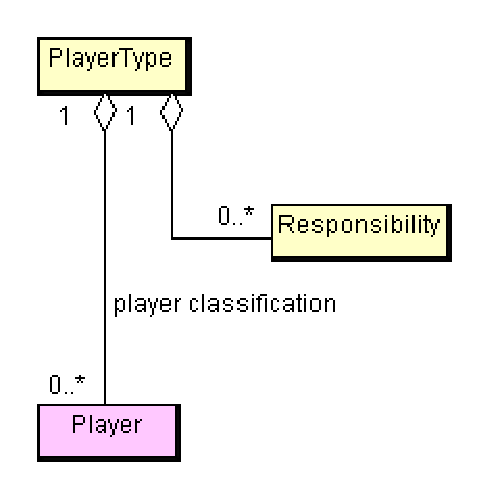
\includegraphics[width=0.4\textwidth]{images/thespian/player-model}
	\caption{The Player model}
	\label{figure:thespian-player-model}
\end{figure}

\subsubsection*{Player and Player Type}

% Type-token distinction - player
To facilitate the type-token distinction for players, \textit{Thespian} contains concepts for modelling both a \textit{player type} and a \textit{player token}: \textit{Player type} and \textit{Player}.

% Player type
\textit{Player type} (also called \textit{Player class}) is a class of players sharing the same capabilities; it is a design-time entity.
% Player type - state
It has a set of \textit{responsibilities} defining its capabilities when playing a role.
% Player type - behaviour
It can be instantiated to yield a \textit{player}\comments{FO}.

% Player
\textit{Player} is an actual player in a running MAS; it is a run-time entity.
% Player - state
It is classified by a \textit{player type} which specifies its .
% Player - note
Note that despite begin a run-time entity, a player has to be declared at design-time, because in this thesis, we do not consider creating and destroying players at run-time.
When declared at design-time, the player is created at MAS start-up.

\subsubsection*{Responsibility}

% Responsibility
\textit{Responsibility} is an operation a player playing a role \textit{must} execute as a result of playing that role; it is a design-time entity.
% Responsibility - state
A \textit{Responsibility} can provide an argument to a player after its invocation (but before its execution), in which case the argument type (a Java type) has to be specified.
Also it can request a return value from the player after its execution, in which case the return value type (a Java type) has to be specified.

%%%%%%%%%%%%%%%%%%%%%%%%%%%%%%%%%%%%%%%%%%%%%%%%%%%%%%%%%%%%%%%%%%%%%%%%%%%%%%%%
\subsection{Protocol Model}

% Protocol model - usage
The \textit{Protocol model} (figure~\ref{figure:thespian-protocol-model}) contains abstractions whose instances represent interaction protocols between a player and an organization or role, and among roles themselves.

% Figure: Thespian - Protocol metamodel
\begin{figure}[ht]
	\centering
	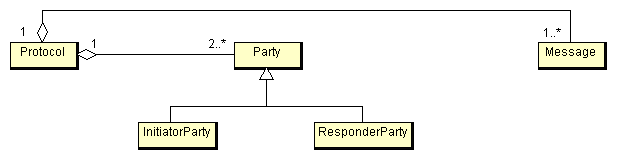
\includegraphics[width=0.8\textwidth]{images/thespian/protocol-model}
	\caption{The Protocol model}
	\label{figure:thespian-protocol-model}
\end{figure}

\subsubsection*{Protocol}

% Protocol
An \textit{Interaction protocol} (or simply \textit{Protocol}) is an institutionalized pattern of interaction (communication) between two or more roles within an organization; it is a design-time entity.
It defines parties involved in the interaction and messages exchanged in the communication.

% Scenario
A realization of an interaction protocol is an \textit{interaction scenario}---a sequence of actions performed (messages exchanged) by two or more positions within an organization; a scenario is a purely run-time entity.
In other words, a protocol is a framework and a scenario (is) one of its possible instantiations.
Since scenarios are usually not explicitly modelled\footnote{Scenarios can be explicitly modelled in snapshots.}, \textit{Thespian} does not contain the concept of an \textit{Interaction scenario}.

% Type-token distinction - protocol
The theme of type-token distinction is at play here: instances of \textit{Protocol} model \textit{protocol types} and instances of \textit{Scenario} represent \textit{protocol tokens}.

\subsubsection*{Party}

% Party - definition
A \textit{Party} is a role involved in a protocol; it is a design-time entity.
A relationship between roles and protocols is a many-to-many one---a role can participate in multiple protocols and at least two different roles have to take part in a protocol.
A party is a reification (embodiment) of this relationship.
% Initiator party & Responder party
A \textit{Party} is either an \textit{Initiator party}---one that initiates the protocol---or a \textit{Responder party}---one that responds to the initiated protocol.

\subsubsection*{Message}

A \textit{Message} is a piece of information exchanged between two parties in a protocol; it is a design-time entity.

%%%%%%%%%%%%%%%%%%%%%%%%%%%%%%%%%%%%%%%%%%%%%%%%%%%%%%%%%%%%%%%%%%%%%%%%%%%%%%%%
\subsection{Design-Time Model}	

% Design-time model - usage
The \textit{Design-time model} (figure~\ref{figure:thespian-design-time-model}) contains concepts whose instances model the design-time MAS entities.
These entities, as their name suggests, are created and/or modified at design-time by the MAS designer, and they constitute the \textit{MAS specification}.

% Figure: Thespian - Compie-time model
\begin{figure}[ht]
	\centering
	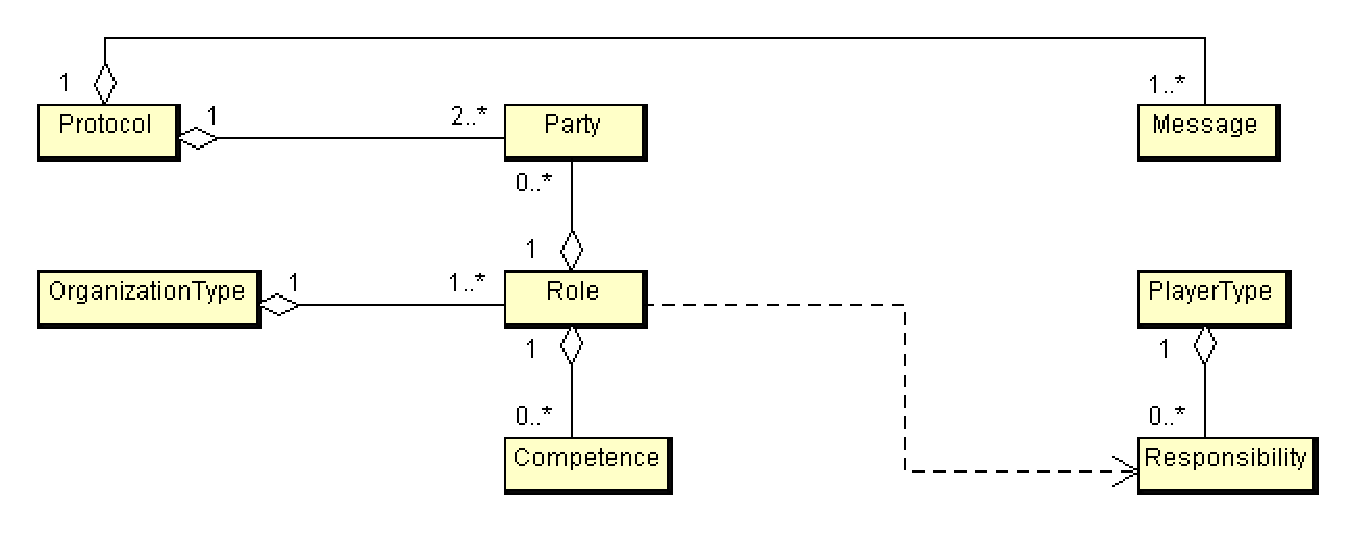
\includegraphics[width=0.8\textwidth]{images/thespian/design-time-model}
	\caption{The Design-time model}
	\label{figure:thespian-design-time-model}
\end{figure}

%%%%%%%%%%%%%%%%%%%%%%%%%%%%%%%%%%%%%%%%%%%%%%%%%%%%%%%%%%%%%%%%%%%%%%%%%%%%%%%%
\subsection{Run-Time Model}

% Run-time model - usage
The \textit{Run-time model} (figure~\ref{figure:thespian-run-time-metamodel}) contains constructs that model the run-time MAS entities.
These entities, as their name implies, are created and/or modified at run-time by the MAS itself, and they make up the \textit{MAS manifestation}.
They models of MAS manifestations are also referred to as \textit{snapshots}.

% Figure: Thespian - Run-time model
\begin{figure}[ht]
	\centering
	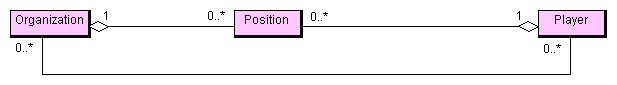
\includegraphics[width=0.8\textwidth]{images/thespian/run-time-model}
	\caption{The Run-time model}
	\label{figure:thespian-run-time-metamodel}
\end{figure}

%%%%%%%%%%%%%%%%%%%%%%%%%%%%%%%%%%%%%%%%%%%%%%%%%%%%%%%%%%%%%%%%%%%%%%%%%%%%%%%%
\subsection{Integrated Static Model}

Figure~\ref{figure:thespian-integrated-metamodel} shows the integrated \textit{Thespian} static model.

% Figure: Thespian static model
\begin{figure}[ht]
	\centering
	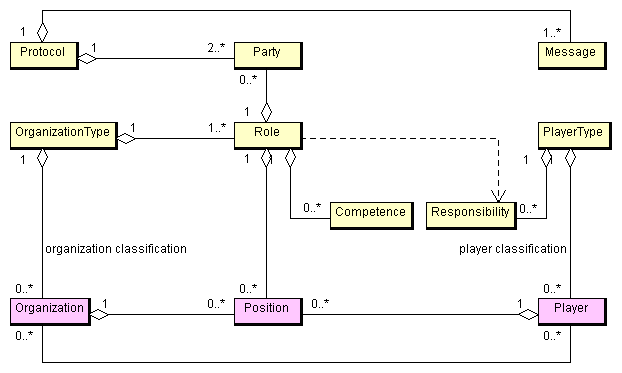
\includegraphics[width=0.8\textwidth]{images/thespian/thespian-metamodel}
	\caption{The \textit{Thespian} static model}
	\label{figure:thespian-integrated-metamodel}
\end{figure}

% Key property of Thespian - no association between Role and Player type
We would like to emphasize what we perceive as key property of \textit{Thespian}: there is no association between \textit{Role} and \textit{Player type}, no link between a specific \textit{role} and a particular \textit{player type}.
This means that there is no \textit{design-time} dependency between roles and player types; all connections arise at \textit{run-time} and happen between \textit{positions} and \textit{players}.